% Figura cuerpo B2: la demolición del menú: curvas de corto plazo, tasa natural y vertical de largo plazo
\documentclass[tikz,border=3pt]{standalone}
\usepackage[T1]{fontenc}
\usepackage[utf8]{inputenc}
\usetikzlibrary{arrows.meta,calc,positioning}
\begin{document}
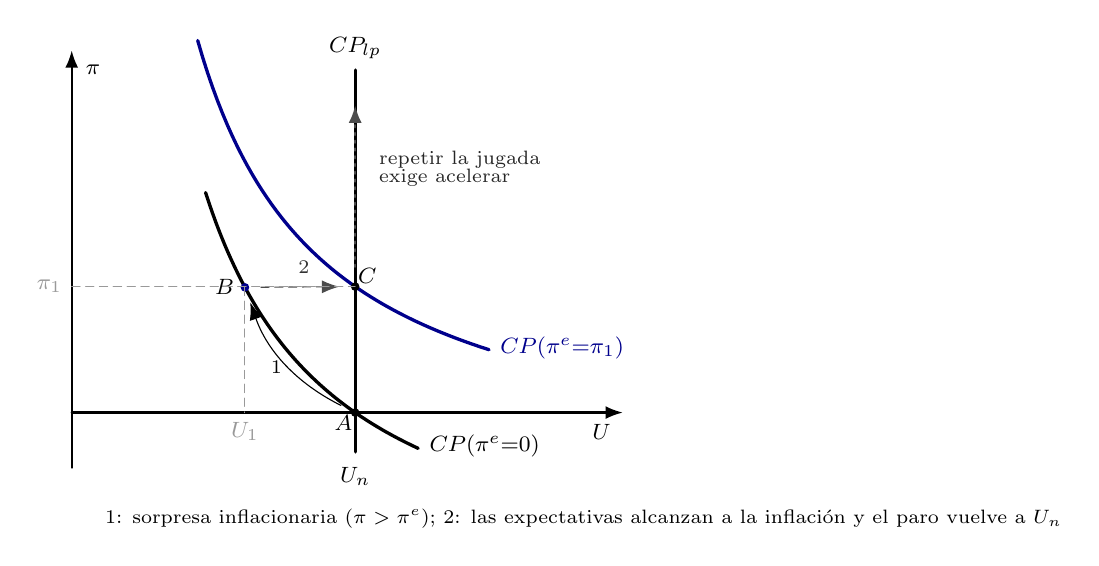
\begin{tikzpicture}[>={Latex[length=2.2mm]}, line cap=round, font=\footnotesize,
  eje/.style={->, thick},
  curva/.style={very thick},
  nueva/.style={very thick, blue!55!black},
  guia/.style={densely dashed, gray!80},
  pto/.style={circle, fill=black, inner sep=1.1pt}]
  \draw[eje] (0,-0.7) -- (0,4.6) node[below right=2pt]{$\pi$};
  \draw[eje] (0,0) -- (7.0,0) node[below left=1pt]{$U$};
  % Vertical de largo plazo
  \draw[curva] (3.6,-0.5) -- (3.6,4.35) node[above]{$CP_{lp}$};
  % Curvas de corto plazo
  \draw[curva, domain=1.7:4.4, samples=60] plot (\x,{9*(1/\x-0.27778)});
  \node[anchor=west] at (4.42,-0.42) {$CP(\pi^{e}{=}0)$};
  \draw[nueva, domain=1.6:5.3, samples=60] plot (\x,{1.6+9*(1/\x-0.27778)});
  \node[anchor=west, blue!55!black] at (5.32,0.82) {$CP(\pi^{e}{=}\pi_1)$};
  % Danza A -> B -> C
  \node[pto] (A) at (3.6,0) {};
  \node[below left=-2pt of A, inner sep=1pt] {$A$};
  \node[pto, fill=blue!55!black] (B) at (2.2,1.59) {};
  \node[left=1pt of B, inner sep=1pt] {$B$};
  \node[pto] (C) at (3.6,1.6) {};
  \node[above right=-2pt of C, inner sep=1pt] {$C$};
  \draw[->, shorten >=4pt, shorten <=4pt] (A) to[bend left=22] (B);
  \node at (2.6,0.58) {\scriptsize 1};
  \draw[->, densely dashed, gray!60!black, shorten >=4pt, shorten <=4pt] (B) -- (C);
  \node[gray!40!black] at (2.95,1.84) {\scriptsize 2};
  \draw[->, dotted, thick, gray!60!black] (3.6,1.85) -- (3.6,3.9);
  \node[align=left, anchor=west, gray!30!black] at (3.78,3.1) {\scriptsize repetir la jugada\\[-3pt]\scriptsize exige acelerar};
  \draw[guia] (0,1.6) node[left]{$\pi_1$} -- (3.6,1.6);
  \draw[guia] (2.2,1.59) -- (2.2,0) node[below]{$U_1$};
  \node[below=2pt] at (3.6,-0.5) {$U_n$};
  \node[align=left, anchor=north west] at (0.3,-1.1) {\scriptsize 1: sorpresa inflacionaria ($\pi>\pi^{e}$); 2: las expectativas alcanzan a la inflación y el paro vuelve a $U_n$};
\end{tikzpicture}
\end{document}
